%Config
\documentclass[12pt,twoside]{report}
\usepackage[spanish,es-tabla]{babel}
\usepackage[a4paper]{geometry}

\usepackage{graphicx}               % Para incluir imágenes
\usepackage{amsmath}                % Para el manejo de matemáticas
\usepackage{url}
\usepackage{array}					% Para ajustar el texto en la celda
\usepackage{xcolor}
\usepackage{amssymb}
\usepackage{algorithm}
\usepackage{algpseudocode}
\usepackage{listings}
\usepackage{enumitem}


\lstdefinestyle{pythonstyle}{
	language=Python,
	basicstyle=\ttfamily\small,
	keywordstyle=\color{blue}\bfseries,
	commentstyle=\color{gray},
	stringstyle=\color{red},
	numbers=left,
	numberstyle=\tiny,
	stepnumber=1,
	frame=single,
	backgroundcolor=\color{lightgray!20},
	tabsize=4,
	showstringspaces=false,
	breaklines=true,        % Permite que las líneas largas se dividan
	linewidth=\linewidth    % Autoajuste al ancho del contenedor
}

% Opening
\title{Mexican Axolotl Optimization}
\author{Erick Jesse Angeles López}


% Definir un comando para palabras clave
\newcommand{\keywords}[1]{%
	\begin{center}
		\textbf{Palabras clave:} #1
	\end{center}
}

\renewcommand{\baselinestretch}{1}
\setcounter{page}{1}
\setlength{\textheight}{21.6cm}
\setlength{\textwidth}{14cm}
\setlength{\oddsidemargin}{1cm}
\setlength{\evensidemargin}{1cm}
\pagestyle{myheadings}
\thispagestyle{empty}
\markboth{\small{Ángeles López Erick Jesse}}{\small{Mexican Axolotl Optimization}}
\date{}

\begin{document}
	
	\begin{center}
		
		% Contenido izquierdo - Imagen
		\begin{minipage}{0.17\textwidth}
			\centering
			
\includegraphics[width=0.7\textwidth]{img/cic_logo.png} % Ajusta esta línea
		\end{minipage}
		\begin{minipage}{.55\textwidth}
			\centering
			{\Large Instituto Politécnico Nacional}\\
			{\Large Escuela Superior de Cómputo}\\
			{\Large Centro de Investigación en Computación}
		\end{minipage}
		\begin{minipage}{0.17\textwidth}
			\centering
			
\includegraphics[width=0.9\textwidth]{img/escom_logo} % Ajusta esta línea
		\end{minipage}			
	\end{center}
	
	
	\centerline{\bf Ingeniería en Inteligencia Artificial, Mexican Axolotl Optimization}
	
	\centerline{\bf Fecha: \today}
	
	\centerline{}
	
	%\centerline{}
	
	
	\begin{center}
		\Large{\textsc{Mexican Axolotl Optimization}} 
	\end{center}
	\centerline{}
	\centerline{\bf {\textit{Presenta}}}
	\centerline{}
	\centerline{\bf {Angeles López Erick Jesse\footnote{eangelesl1700@alumno.ipn.mx}}}
	\centerline{}
	\centerline{}
	\centerline{\bf {Disponible en:}}
	\centerline{\text{\url{github.com/JesseAngeles/Metaheuristicas}}}
	

	\newtheorem{Theorem}{\quad Theorem}[section]
	
	\newtheorem{Definition}[Theorem]{\quad Definition}
	
	\newtheorem{Corollary}[Theorem]{\quad Corollary}
	
	\newtheorem{Lemma}[Theorem]{\quad Lemma}
	
	\newtheorem{Example}[Theorem]{\quad Example}
	
	\bigskip
	
	\bigskip
	
	\begin{center}\textbf{Resumen}\end{center}
	
	RESUMEN \\ 
	
	En esta practica se describe el comportamiento, las partes esenciales, configuraciones, implementación y comparación de resultados de \textit{Mexican Axolotl Optimization}, como un algoritmo bioinspirado utilizado para la búsqueda de óptimos globales en problemas de optimización.
	
	\keywords{Axolote, Evolución, Resultado óptimo}
	
	\clearpage
	
	\tableofcontents
	\clearpage
	
\chapter*{Introducción}
\addcontentsline{toc}{chapter}{Introducción}
	
	\textit{Mexican Axolotl Optimization} (\textit{MAO}) es una técnica de optimización bioinspirada que toma como referencia las características biológicas y comportamentales únicas del axolote mexicano. Esta especie se destaca por su notable capacidad de regeneración de órganos, su habilidad para el camuflaje, así como por su complejo sistema reproductivo que involucra poblaciones diferenciadas de machos y hembras, además de mecanismos de cruza genómica. Estas propiedades naturales han servido de modelo para diseñar un algoritmo que simula procesos de supervivencia, adaptación y evolución, proporcionando un enfoque novedoso para resolver problemas de optimización complejos \cite{mao}.
	
	En esta práctica, el objetivo principal es comprender en profundidad el funcionamiento interno de \textit{MAO} y evaluar cómo sus principales metaparámetros influyen en su desempeño. Entre estos parámetros se encuentran la tasa de “aprendizaje”, que controla la velocidad de adaptación del algoritmo; la probabilidad de daño y la probabilidad de sanación, que simulan procesos de deterioro y recuperación biológica; y el tamaño del torneo para cruza, que determina la presión selectiva durante la combinación genética. Estos elementos representan etapas esenciales del algoritmo y su correcta configuración es fundamental para lograr un rendimiento óptimo.
	
	Esta exploración no solo contribuye a afianzar los fundamentos teóricos que sustentan \textit{MAO}, sino que también permite desarrollar un criterio práctico para la selección y ajuste de sus componentes, de modo que se adapten de manera eficiente a distintos tipos de problemas. De esta manera, se busca potenciar la aplicabilidad del algoritmo y facilitar su implementación en contextos reales donde la optimización es un desafío constante.

	\chapter{Mexican Axolotl Optimization}

Los dioses mexicas se reunieron en Teotihuacan para crear el universo ofreciendo su propia vida en sacrificio. Dioses como Huitzilopochtli, Xochipilli y Tezcatlipoca tomaron el sacrificio, sin embargo, Xolotl, victima del miedo, huyo del ritual. 

Xolotl se transformo en múltiples criaturas para evitar se atrapado por el viento, se transformo en diferentes criaturas pero seguía siendo encontrado, por lo que opto por arrojarse al lago convirtiéndose en un anfibio con branquias en forma de cuernos, un axolote. Pudo sobrevivir algunos días en el lago pero finalmente fue atrapado por el viento y llevado al ritual para dar movimiento al universo \cite{leyenda}.

\section{Modelo natural}

El axolote mexicano o \textit{Ambystoma mexicanum} es una especie endémica del lago de Xochimilco, son salamandras que nunca superan su fase larvaria. Tiene branquias que brotan de su cabeza, patas palmeadas, una aleta dorsal, cola, pulmones funcionales, camuflaje y una sonrisa.

Los axolotes son un tema de investigación por biólogos dado a su capacidad de regenerar extremidades y órganos sin cicatrices permanentes \cite{axolote}.

\section{Modelo artificial}

 El algoritmo \textit{Mexican Axolotl Optimization} (\textbf{MAO}) busca imitar el comportamiento de estos anfibios para encontrar la mejor solución en un espacio de búsqueda dadas las siguientes analogías:
 
 \begin{itemize}
 	\item Los ajolotes son soluciones de problemas y sus órganos y extremidades las dimensiones de la solución.
 	\item El lago en donde viven es el espacio de búsqueda.
 	\item El camuflaje del axolote, cuya efectividad depende del estado de búsqueda, determina la capacidad de sobrevivir, es decir, su aptitud.
 \end{itemize}
 
 En otras palabras, sea $O$ un problema de optmización numerica cuyas elementos sea vectores de dimensión $D$ acotados en el rango $[\min_i, \max_i]$, los axolotes representan un conjunto de soluciones de tamaño $np$: $P = \{ S_1, \dots, S_{np} \}$ donde $O(S_j) \in \mathbb{R} \; \forall j \in \{1, \dots,  np\}$.
 
 El algoritmo MAO es un proceso iterativo de 4 etapas definida por el acronimo \textit{TIRA}: transición de larva a adulto (\textit{Transition}), lesión y restauración \textit{Injury and restoration}, reproducción (\textit{Reproduction}) y variedad (\textit{Assortment}).
 
 \subsection{Transition}
 
 La población de axolotes se inicia de manera aleatoria y a cada individuo se le asigna un genero, obteniendo dos subconjuntos. Los individuos de cada grupo transicionan en el agua de larvas a adultos ajustando el color de las partes de su cuerpo para parecerse mas al mejor de cada grupo, como se muestra en el algoritmo \ref{alg:transition}
 
 \begin{algorithm}
 	\caption{Transition \\
 	\textbf{Input} constante de diferenciación $\alpha$, Población $P$, Función de optimización $O$ \\
 	\textbf{Output}  Población actualizada $P'$} 
 	\begin{algorithmic}[1]
 		\State El mejor axolote: $p_{best} = Best(P)$
 		\For{$p_j \in P $}
 			\State Probabilidad inversa de transición: $pp_j = \frac{O(p_j)}{\sum O(p_i)}$
 			\If{$pp_j < r$}
 				\State Se aproxima al mejor: $p_{j,i} = p_{j,i} + (p_{best, i} - p_{j,i}) \cdot \alpha $
 			\Else
 				\State Se mueve de forma aleatoria: $p_{j,i} = \min_i + (\max_i - \min_i) * r_i$
 			\EndIf
 		\EndFor 
 	\end{algorithmic}
 	\label{alg:transition}
 \end{algorithm}
 
 La habilidad de los ajolotes de cambiar de color esta limitada, por lo que unicamente se aproximan a la nueva solución, ya que no se busca que se adapten de forma perfecta al mejor de ellos. Cuando los individuos son difieren mucho de la mejor solución, medida que se obtiene con la probabilidad inversa, se mueven de manera aleatoria para explorar el espacio.
 
 \subsection{Injury and restoration}
 
 Mientras los axolotes se mueven en el agua pueden sufrir accidentes y ser lastimados. En esta fase los ajolotes pierden partes que posteriormente regeneran de forma aleatoria, para esto, se consideran ambas probabilidades donde la primera actuá sobre los axolotes que serán lastimados y la segunda sobre las partes del cuerpo que serán regeneradas, esto se aplica para ambos grupos como se muestra en el algoritmo \ref{alg:injury}.
 
  \begin{algorithm}
 	\caption{Injury and Restoration \\
 		\textbf{Input} Población $P$, probabilidad de daño $dp$, probabilidad de regeneración $rp$ \\
 		\textbf{Output}  Población actualizada $P'$} 
 	\begin{algorithmic}[1]
 		\For{ $p_j \in P$}
 			\If{$r \leq dp$}
 				\For{$i \in D$}
 					\If{$r \leq rp$}
 						\State $p_{j,i} = \min_i + (\max_i - \min_i) * r_i$
 					\EndIf
 				\EndFor
 			\EndIf
 		\EndFor
 	\end{algorithmic}
 	\label{alg:injury}
 \end{algorithm}
 
 \subsection{Reproduction and Assortment}
 
 Los machos y las hembras se reproducen dejando un par de huevos que contienen una mezcla del material genético de los padres de forma uniforme. Se genera una cadena aleatoria de tamaño $D$ y si es un 0 el primer hijo hereda el gen del padre y el dos de la madre, si es un 1 el primer hijo hereda del gen de la madre y el dos del padre, como se muestra en la figura \ref{fig:uniform}.

 \begin{figure}[H]
 	\centering
 	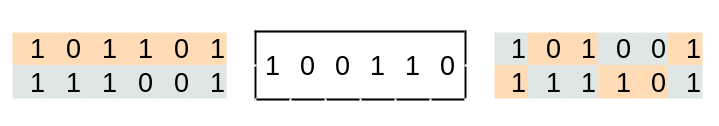
\includegraphics[width=0.75\linewidth]{img/cross_uniform.png}
 	\caption{Cruza uniforme}
 	\label{fig:uniform}
 \end{figure}
 
 El algoritmo \ref{alg:resproduction} selecciona, entre un rango de machos, con quien reproducirse mediante un torneo de tamaño $k$ con cada hembra, cuyos huevos heredan el material genético. Finalmente, entre los 4 individuos se seleccionan los dos mejores y se les asigna el genero de hembra y macho al primero y segundo mejor respectivamente.
 
   \begin{algorithm}[H]
 	\caption{Reproduction \\
 		\textbf{Input} Población $P$, probabilidad de daño $dp$, probabilidad de regeneración $rp$ \\
 		\textbf{Output}  Población actualizada $P'$} 
 	\begin{algorithmic}[1]
 		\For{ $f \in F$}
 			\State $m = \{Best(MC) | MC \subset M \land |MC| = k\}$
 			\State egg$_1$
 			\State egg$_2$
 			\For{$i \in D$}
 				\If{$r \leq 0.5$}
 					\State huevo$_{1,i} = m_i$
 					\State huevo$_{2,i} = f_i$ 
 				\Else
 					\State huevo$_{1,i} = f_i$
 					\State huevo$_{2,i} = m_i$ 
 				\EndIf
 			\EndFor
 		\EndFor
 		\State $V=Sort(function= O, \{ f, m, \text{huevo}_1, \text{huevo}_2 \})$
 		\State $f = V[0]$
 		\State $m = V[1]$
 	\end{algorithmic}
 	\label{alg:resproduction}
 \end{algorithm}
 

\section{Ventajas}

La técnica \textit{Mexican Axolotl Optimization} (\textit{MAO}) presenta varias ventajas importantes:

\begin{itemize}
	\item \textbf{Inspiración biológica robusta:} Su diseño se basa en procesos naturales probados, como la regeneración y adaptación, lo que permite un enfoque balanceado entre exploración y explotación.
	\item \textbf{Capacidad de adaptación dinámica:} Gracias a sus parámetros como la probabilidad de daño y sanación, el algoritmo puede adaptarse a distintos escenarios y escapar de óptimos locales.
	\item \textbf{Manejo efectivo de poblaciones heterogéneas:} La diferenciación entre machos y hembras y la cruza genómica permiten mantener diversidad genética, lo que mejora la búsqueda global.
	\item \textbf{Versatilidad:} Puede ser aplicado a problemas de optimización continua, compleja y de alta dimensión.
\end{itemize}

\section{Desventajas}

Sin embargo, \textit{MAO} también presenta algunas limitaciones:

\begin{itemize}
	\item \textbf{Sensibilidad a la configuración:} La selección incorrecta de metaparámetros puede degradar significativamente el rendimiento del algoritmo.
	\item \textbf{Costo computacional:} El manejo de poblaciones grandes y múltiples iteraciones puede resultar en tiempos de cómputo elevados, especialmente para problemas complejos.
	\item \textbf{Falta de garantías teóricas:} Como muchas heurísticas bioinspiradas, no ofrece garantías matemáticas de convergencia al óptimo global.
	\item \textbf{Implementación compleja:} La modelación de procesos biológicos complejos puede dificultar la implementación y ajuste del algoritmo para usuarios sin experiencia.
\end{itemize}

\section{Aplicaciones}

El algoritmo \textit{Mexican Axolotl Optimization} ha demostrado ser útil en diversas áreas de optimización, tales como:

\begin{itemize}
	\item Optimización de funciones continuas y no lineales. Resuelve problemas complejos con múltiples variables y restricciones.
	\item Selección de parámetros óptimos en modelos de machine learning.
	\item Inspiración para simulaciones en biología computacional y estudios de dinámica poblacional.
\end{itemize}
 
 
	\chapter{Problemas}

\section{Knapsack problem}

Dado un conjunto de $n$ ítems \[I = \{1,2, \dots, n \}\] Donde cada ítem $i$ tiene un valor $v_i \geq 0$ y un peso $w_i \geq 0$ y dada una mochila con capacidad máxima $W$, se busca seleccionar un subconjunto de ítems que maximice el valor total sin exceder la capacidad.

Podemos representar los elementos dentro de la mochila como un vector binario: 
\[ x = (x_1, x_2, \dots , x_n) \; \text{con } x_i \in \{0, 1\} \]
Donde:
\begin{itemize}
	\item $x_i = 0$ si el ítem no esta en la mochila
	\item $x_i = 1$ si el ítem si esta en la mochila
\end{itemize}

Para calcular el valor $v(x)$ y el peso $w(x)$ de la mochila sumamos los valores que si se encuentren dentro de ella:
\begin{gather*}
	v(x) = \sum_{i = 1}^{n} v_i x_i \\
	w(x) = \sum_{i = 1}^{n} w_i x_i 
\end{gather*}

El objetivo, es encontrar el mayor $v(x)$ siempre que el peso $w(x)$ no exceda el peso máximo $W$. 

\begin{itemize}
	\item El conjunto de estados posibles son todas las cadenas binarias de tamaño $n$: \[ S = \{ x \in \{ 0, 1  \}^n \} \]
	
	\item El estado inicial puede ser cualquier cadena de tamaño $n$ cuyo peso no exceda el peso máximo: \[ s_0 = \{x \in \{0,1\}^n | w(x) \leq W \} \]
	
	\item Se busca maximizar el valor de la mochila. La función objetivo suma los valores de los objetos dentro de la mochila. Si el peso de la mochila excede el limite, entonces se le asigna una ganancia negativa. 
	\[
	f(x) =
	\begin{cases} 
		v(x), & \text{si } w(x) \leq W \\ 
		W - w(x), & \text{si } w(x) > W
	\end{cases}
	\]
	
	Se le asigna la diferencia del peso máximo menos el peso actual (Dando un numero negativo). Esto con el objetivo de que, si por alguna razón esa es la mejor solución actual, sepa encontrar una mejor solución disminuyendo esa diferencia.
	
	\item Entonces, un estado $x_j$ es un estado final si genera mayor aptitud en comparación de los demás $x_i$ generados y tiene una aptitud no negativa: \[ f(x_j) \geq 0 \land f(x_j) \geq f(x_i) \; \forall x_i \in S\]
	
	\item La operación que genere genere el vecino sera \textit{Bit flip} que intercambia un 0 por un 1 y viceversa en una posición aleatoria $i$).
	
	\[
	B(x_i) =
	\begin{cases} 
		1, & \text{si } x_i = 0 \\ 
		0, & \text{si } x_i = 1 \\
	\end{cases}
	\]
	
\end{itemize}

\section{Minimizar la función}

Obtener los mínimos de la función \[ f(x) = \ \sum_{i = 1}^{D} x_i^2, \; \text{ con } -10 \geq x_i \geq 10 \].

Dado un vector de $D$ números en el rango de $[-10, 10]$, se busca obtener el valor mínimo del sumatoria  de sus cuadrados.

\begin{itemize}
	\item El conjunto de estados posibles son todas las cadenas de enteros en dicho intervalo: \[ S = \{ x \in [-10, 10]^n \} \]
	
	\item El estado inicial se genera de forma arbitraria como un vector de $D$ números en el rango establecido $[-10, 10]$
	
	\item La función objetivo unicamente considera los valores dentro del propio vector: \[f(x) \]
	
	\item Un estado de aceptación $x_j$ es aquel que produzca el menor valor de aptitud en la función comparando con los demás $x_i$ generados: \[ f(x_j) \leq f(x_i) \; \forall x_i \in S\] 
	
	\item La operación que genere los vecinos puede tener multiples interpretaciones. Para este problema se asume un espacio circular donde $-10$ es el consecutivo del $10$ y que $\forall d_i \in D, d_i \in \mathbb{Z}$.  Entonces, los vecinos de $d_i$ son los números consecutivos, es decir $d_{i-1}$ y $d_{i+1}$.
	
	La operación sera entonces:
	\[ d_i = min(f(d_{i-1}), f(d_i), f(d_{i+1})) \]	
\end{itemize}

\section{Problemas de optimización CEC 2017}

En el documento \cite{cec} se presentan una serie de problemas sobre optimización numérica de parámetros reales. En este reporte se analizan las 10 primeras funciones que cumplen con la siguiente definición:
\begin{itemize}
	\item Todas las funciones son problemas de minimización definidos de la siguiente manera:
	\[ min f(x), \; x = [x_1, x_2, \dots, x_D]^T \]
	Donde:
	\begin{itemize}
		\item $x$ es el vector de variables de dimensión $D$ que representa la solución del problema.
		\item $D$ es el numero de dimensiones del problema.
	\end{itemize}
	
	\item El óptimo global (la mejor solución) se encuentra desplazada del origen para evitar respuestas que asumen que la respuesta esta cerca del origen:
	\[ o = [ o_1, o_2, \dots, o_D ]^T \]
	Donde $o$ es el vector del optimo global desplazado.
	
	El valor óptimo se distribuye de manera aleatoria en el rango de $o \in [-80, 80]^D$
	
	\item Las funciones son escalables, es decir, el numero de dimensiones $D$ puede variar.
	
	\item El rango de búsqueda de todas las funciones para las variables se delimita por $x \in [-100, 100]^D$
	
	\item Implementación de matrices de rotación: Las variables interactúan entre ellas para volver el problema más difícil.
	
	\item Para simular problemas reales, las variables se dividen de manera aleatoria en subcomponentes. Cada subcomponente tiene su propia matriz de rotación.
	
\end{itemize}

\subsection{Funciones}

A continuación se definen las 10 primeras funciones.

\subsubsection*{1) Bent Cigar Function}
\[
f(x) = x_1^2 + 10^6 \sum_{i=2}^{D} x_i^2
\]

\subsubsection*{2) Zakharov Function}
\[
f(x) = \sum_{i=1}^{D} x_i^2 + \left( 0.5 \sum_{i=1}^{D} i x_i \right)^2 + \left( 0.5 \sum_{i=1}^{D} i x_i \right)^4
\]

\subsubsection*{3) Rosenbrock's Function}
\[
f(x) = \sum_{i=1}^{D-1} \left[ 100 (x_{i+1} - x_i^2)^2 + (x_i - 1)^2 \right]
\]

\subsubsection*{4) Rastrigin's Function}
\[
f(x) = \sum_{i=1}^{D} \left[ x_i^2 - 10 \cos(2 \pi x_i) + 10 \right]
\]

\subsubsection*{5) Expanded Schaffer's F6 Function}
\[
g(x, y) = 0.5 + \frac{\sin^2(\sqrt{x^2 + y^2}) - 0.5}{(1 + 0.001(x^2 + y^2))^2}
\]

\[
f(x) = \sum_{i=1}^{D-1} g(x_i, x_{i+1})
\]

\subsubsection*{6) Lunacek Bi-Rastrigin Function}
\[
f(x) = \min \left( \sum_{i=1}^{D} (x_i - \mu_0)^2, dD + s \sum_{i=1}^{D} (x_i - \mu_1)^2 \right) 
+ 10 \sum_{i=1}^{D} \left[ 1 - \cos(2 \pi z_i) \right]
\]

\[
\mu_0 = 2.5, \quad \mu_1 = -\sqrt{\frac{\mu_0^2}{d}}
\]

\subsubsection*{7) Non-Continuous Rotated Rastrigin's Function}
\[
f(x) = \sum_{i=1}^{D} \left[ z_i^2 - 10\cos(2\pi z_i) + 10 \right]
\]

\[
z_i = \text{Tosz}(\text{Tasy}(x_i))
\]

\subsubsection*{8) Levy Function}
\[
f(x) = \sin^2(\pi w_1) + \sum_{i=1}^{D-1} (w_i - 1)^2 \left[ 1 + 10\sin^2(\pi w_i + 1) \right] + (w_D - 1)^2 \left[ 1 + \sin^2(2\pi w_D) \right]
\]

\[
w_i = 1 + \frac{x_i - 1}{4}
\]

\subsubsection*{9) Modified Schwefel's Function}
\[
f(x) = 418.9829 D - \sum_{i=1}^{D} x_i \sin(\sqrt{|x_i|})
\]

\subsubsection*{10) High Conditioned Elliptic Function}
\[
f(x) = \sum_{i=1}^{D} 10^{6 \frac{i-1}{D-1}} x_i^2
\]

Cuyas graficas se observan en la figura \ref{fig:cec}

\begin{figure}[H]
	\centering
	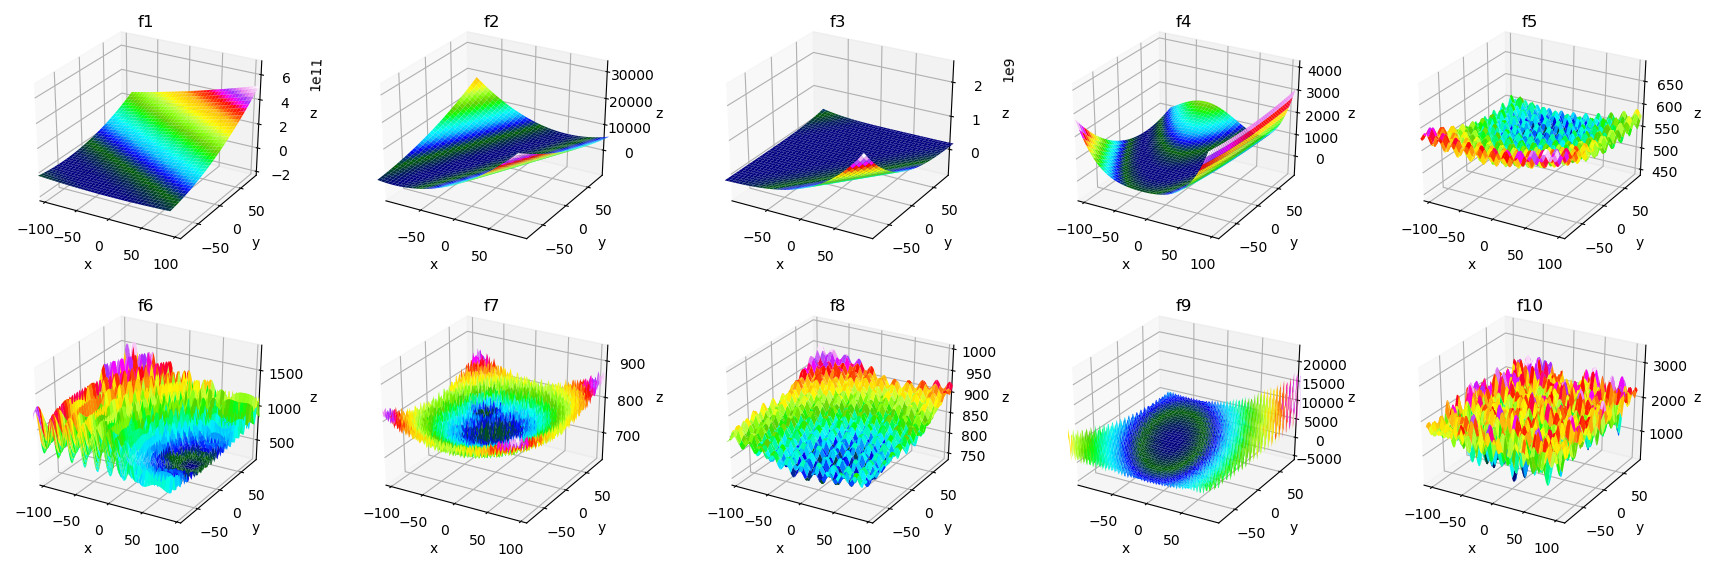
\includegraphics[width=1\linewidth]{img/cec}
	\caption{Superficies ploteadas de las 10 primeras funciones para dos dimensiones \cite{plot}}
	\label{fig:cec}
\end{figure}
	\chapter{Codigo}

\section{Problem}

Los problemas a optimizar siguen una mista estructura. Dado esto, se optó por diseñar una clase que generaliza el problema y permite y facilita la definición de nuevos problemas.

El código \ref{lst:problem} incluye los siguientes métodos los cuales deben de ser implementados por sus clases hijas:
\begin{itemize}
	\item \textit{generateInformation}: Función que define la información necesaria para calcular la función objetivo. La información adicional depende del problema.
	\item \textit{objective}: Función que calcula la utilidad de la solución, si es un problema de minimización tiene que devolver con el signo opuesto. 
	\item \textit{generateInitialSolution}: Función que genera una solución.
	\item \textit{getRandomNeighbour}: Obtiene un vecino de forma aleatoria.
	\item \textit{getNextNeighbour}: Si es necesario manejar indices, esta función permite obtener un vecino tras otro.
	\item \textit{getNeighbours}: Devuelve todos los vecinos.
\end{itemize}

\begin{lstlisting}[style=pythonstyle, label={lst:problem} ,caption={Clase \textit{problem}}]
class Problem(ABC):
  def __init__(self,):
  self.information:Any = {}

  @abstractmethod
  def generateInformation(self, *args, **kwargs) -> None: pass

  @abstractmethod
  def objective(self, solution: Any) -> float: pass

  @abstractmethod
  def generateInitialSolution(self) -> Any: pass

  @abstractmethod
  def getRandomNeighbour(self, solution:Any) -> Any: pass

  @abstractmethod
  def getNextNeighbour(self, solution:Any, *args, **kwargs) -> Any: pass

  @abstractmethod
  def getNeighbours(self, solution: Any) -> list: pass

  @abstractmethod
  def printInformation(self) -> None: pass
\end{lstlisting}

\subsection{Knapsack problem}

La clase \textit{knapsackProblem} hereda de la clase \textit{Problem} e implementa las siguientes funciones.

La función \ref{lst:kp-gi} genera de manera aleatoria un conjunto de elementos en la mochila con pesos y valores aleatorios en un rango de $[1,10]$. La función \ref{lst:kp-e} calcula la energía del sistema la cual suma todos los pesos y valores de los elementos que se encuentran en la solución, si el peso es menor al capacidad de la mochila entonces devuelve el valor de la mochila, en caso contrario devuelve la diferencia de el peso actual menos la capacidad máxima.

La función \ref{lst:kp-gis} genera soluciones aleatorias de combinaciones y no regresa ninguna de ellas hasta que el peso de la solución sea menor a la capacidad máxima. Finalmente, la función \ref{lst:kp-rn} se encarga de generar un vecino de forma aleatoria, primero selecciona un elemento aleatorio del vector y después lo invierte.  

\begin{lstlisting}[style=pythonstyle, label={lst:kp-gi} ,caption={Función \textit{generateInformation} de Knapsack problem}]
def generate_information(self, items, capacity):
  self.information = {
	"items": items,
	"values": [(random.randint(1,10), random.randint(1, 10)) for _ in range(items)],
	"capacity": capacity
  }
\end{lstlisting}

\begin{lstlisting}[style=pythonstyle, label={lst:kp-e} ,caption={Función \textit{objective} de Knapsack problem}]
def objective(self, solution):
  total_weight = total_value = 0
  for i, selected in enumerate(solution):
    if selected:
      total_weight += self.information["values"][i][0]
  	  total_value += self.information["values"][i][1]
  if total_weight > self.information["capacity"]:
    return self.information["capacity"] - total_weight 
  return total_value
\end{lstlisting}

\begin{lstlisting}[style=pythonstyle, label={lst:kp-gis} ,caption={Función \textit{generateInitialSolution} de Knapsack problem}]
def generateInitialSolution(self):
  return [random.randint(0, 1) for _ in self.information['values']]
\end{lstlisting}

\begin{lstlisting}[style=pythonstyle, label={lst:kp-rn} ,caption={Función \textit{getRandomNeighbour} de Knapsack problem}]
def getRandomNeighbour(self, solution):
  neighbour = solution[:]
  index = random.randint(0, len(solution) - 1)
  neighbour[index] = 1 - int(neighbour[index])
  return neighbour  
\end{lstlisting}

Para el algoritmo genético, no es necesario especificar el resto de funciones.

\subsection{Travel Salesman Problem}

La función \ref{lst:tsp-gi} genera una matriz cuadrada y simétrica de $n$ valores aleatorios en un rango de $[1, 100]$.

La función \ref{lst:tsp-e} calcula la energía del sistema. Dado un vector suma todas las distancias de las ciudades con base en la información generada en \ref{lst:tsp-gi}, el resultado que devuelve es negativo ya que se busca minimizar. La función \ref{lst:tsp-gis} genera un vector de $n$ números consecutivos (representando las ciudades) y cambia las posiciones mediante la función \textit{shuffle}.

Finalmente, la función \ref{lst:tsp-rn} toma dos indices aleatorios diferentes e invierte los valores de dichas posiciones del vector.

\begin{lstlisting}[style=pythonstyle, label={lst:tsp-gi} ,caption={Función \textit{generateInformation} de Travel Salesman Problem}]
def generateInformation(self, cities: int):
  distances = [[0]*cities for _ in range(cities)]

  for i in range(cities):
    for j in range(i, cities):  
      if i == j:
        valor = 0  
      else:
        valor = random.randint(1, 100)
      distances[i][j] = valor
  	  distances[j][i] = valor 

  self.information = {
	"cities" : cities,
	"distances" : distances
  }
\end{lstlisting}

\begin{lstlisting}[style=pythonstyle, label={lst:tsp-e} ,caption={Función \textit{Objective} de Travel Salesman Problem }]
def objective(self, solution):
  distance = 0
  num_cities:int = len(solution)

  for i in range(num_cities):
    current_city = solution[i]
    next_city = solution[(i + 1) % num_cities]  
    distance += self.information['distances'][current_city][next_city]

  return -distance
\end{lstlisting}

\begin{lstlisting}[style=pythonstyle, label={lst:tsp-gis} ,caption={Función \textit{generateInitialSolution} de Travel Salesman Problem}]
def generateInitialSolution(self):
  solution =  list(range(self.information['cities']))
  random.shuffle(solution)
  return solution   
\end{lstlisting}

\begin{lstlisting}[style=pythonstyle, label={lst:tsp-rn} ,caption={Función \textit{getRandomNeighbour} de Travel Salesman Problem}]
def getRandomNeighbour(self, solution):
  neighbour = solution[:]
  i = j = random.randint(0, len(solution) - 1)
  while j == i:
    j = random.randint(0, len(solution) - 1)
  neighbour[i], neighbour[j] = neighbour[j], neighbour[i]

  return neighbour
\end{lstlisting}

\subsection{Sum function Problem}

La función \ref{lst:sfp-gi} unicamente define el tamaño del vector y los rangos de valores. por otro lado, la función \ref{lst:sfp-e} calcula la energía del sistema dada por la suma de los cuadrados, dado que es una función de minimización se invierte el signo.

La función \ref{lst:sfp-gis} genera un vector de $n$ elementos aleatorios en los rangos definidos, mientras que la función \ref{lst:sfp-gn} suma  o resta en uno a un elemento aleatorio del vector (dado que se considera una configuración circular, se ajusta el valor si el nuevo valor no se encuentra en el rango).

\begin{lstlisting}[style=pythonstyle, label={lst:sfp-gi} ,caption={Función \textit{generateInformation} de SumFunctionProblem}]
def generateInformation(self, size: int, min: int, max: int):
  self.information = {
	"size": size,
	"min": min,
	"max": max
  }
\end{lstlisting}

\begin{lstlisting}[style=pythonstyle, label={lst:sfp-e} ,caption={Función \textit{objective} de SumFunctionProblem}]
def objective(self, solution):
  total_sum:float = 0

  for val in solution:
    total_sum += val**2

  return -total_sum
\end{lstlisting}

\begin{lstlisting}[style=pythonstyle, label={lst:sfp-gis} ,caption={Función \textit{generateInitialSolution} de SumFunctionProblem}]
def generateInitialSolution(self):
  solution = [random.randint(self.information['min'], self.information['max']) for _ in range(self.information['size'])]
  return solution
\end{lstlisting}

\begin{lstlisting}[style=pythonstyle, label={lst:sfp-gn} ,caption={Función \textit{getRandomNeighbour} de CEC 2017}]
def getRandomNeighbour(self, solution):
  neighbour = solution[:]
  index = random.randint(0, len(solution) - 1)
  sign = random.choice([-1 , 1])
  neighbour[index] += sign

  if neighbour[index] > self.information['max']:
    neighbour[index] = self.information['min']

  if neighbour[index] < self.information['min']:
	neighbour[index] = self.information['max']

  return neighbour
\end{lstlisting}

\subsection{CEC 2017}

La función \ref{lst:cec-gi} define la función a optimizar, los rangos de valores, el tamaño de la dimensión y la tasa de cambio (ya que la solución es real). Por otro lado, la función \ref{lst:cec-e} calcula la energía del sistema dados los parámetros ya definidos.

La función \ref{lst:cec-gis} genera un vector de la dimensión definida restringida por la información adicional definida, mientras que la función \ref{lst:cec-gn} suma  o resta en \textit{alpha} a un elemento aleatorio del vector.

\begin{lstlisting}[style=pythonstyle, label={lst:cec-gi} ,caption={Función \textit{generateInformation} de CEC 2017}]
def generateInformation(self, function: callable, low:int, high:int, dimention:int, alpha:int):
  self.information = {
	"function": function,
	"low" : low,
	"high": high,
	"dimention": dimention,
	"alpha": alpha
  }
\end{lstlisting}

\begin{lstlisting}[style=pythonstyle, label={lst:cec-e} ,caption={Función \textit{objective} de CEC 2017}]
def objective(self, solution):
  return - self.information["function"]([solution])[0]
\end{lstlisting}

\begin{lstlisting}[style=pythonstyle, label={lst:cec-gis} ,caption={Función \textit{generateInitialSolution} de CEC 2017}]
def generateInitialSolution(self):
  solution = np.random.uniform(low=self.information["low"],
    high=self.information["high"],
    size=self.information["dimention"]).tolist()

  return solution
\end{lstlisting}

\begin{lstlisting}[style=pythonstyle, label={lst:cec-gn} ,caption={Función \textit{getRandomNeighbour} de CEC 2017}]
def getRandomNeighbour(self, solution):
  neighbour = solution[:]
  index = random.randint(0, len(solution) - 1)
  alpha = random.uniform(-self.information["alpha"], self.information["alpha"])

  neighbour[index] += alpha
  return neighbour
\end{lstlisting}

\section{Metaheuristic}

De igual manera, el se diseña una clase padre \ref{lst:meta} que implemente algunas de las funciones compatibles entre algoritmo genético, \textit{hill climbing} y \textit{simulated annealing}.

Esta clase tiene como parametro la clase \textit{Problem} y define los métodos abstractos \textit{resetProblem} y \textit{optimize} los cuales reinician meta parámetros y evalúan el algoritmo, respectivamente.

Adicionalmente se definen 3 funciones:
\begin{itemize}
	\item \textit{evaluate}: recibe como parámetro una solución y devuelve la aptitud definida por el problema
	
	\item \textit{isBetterSolution}: Compara dos soluciones.
	
	\item \textit{isSameSolution}: Verifica si dos soluciones tiene  la misma aptitud.
\end{itemize}

\begin{lstlisting}[style=pythonstyle, label={lst:meta} ,caption={Clase \textit{Metaheuristic}}]
class Metaheuristic(ABC):
  def __init__(self, problem: Problem):
  self.problem = problem

  @abstractmethod
  def resetProblem(self):
    self.solution = self.problem.generateInitialSolution()
    self.is_best = False

  @abstractmethod
  def optimize(self, *args, **kwargs): pass

  def evaluate(self, state: Any) -> float:
    return self.problem.objective(state)

  def isBetterSolution(self, solution_1: Any, solution_2: Any)-> bool:
    return (self.problem.objective(solution_1) > 
    	self.problem.objective(solution_2)) 

  def isSameSolution(self, solution_1: Any, solution_2: Any) -> bool:
  return (self.problem.objective(solution_1) ==
  	  self.problem.objective(solution_2)) 

  def printSolution(self) -> None:
    print(f'Solution: {self.solution}: {self.evaluate(self.solution)}')

  def getSolution(self) -> Any:
    return self.solution

  def setSolution(self, solution: Any):
    self.solution = solution
\end{lstlisting}

\subsection{Genetic Algorithm}

La clase \textit{GeneticAlgorithm} hereda de la clase \textit{Metaheuristic} e incluye las clases \textit{GASelectionFunctions}, \textit{GACrossoverFunctions}, \textit{GAMutationFunctions} y \textit{GAReplaceFunctions} que se verán mas adelante.

El constructor del código \ref{lst:ga-init} recibe como parametros el problema de optimización y el tamaño de la población. Adicionalmente crea los objetos de las funciones para poder ser accedidas desde esa misma clase y llama la función \ref{lst:ga-rp}, la cual predefine las funciones del algoritmo e inicializa la población.

La función \ref{lst:ga-o} se encarga de encontrar la mejor solución realizando las operaciones de selección, cruza, mutación y reemplazo. Nótese que esta función recibe como parámetro \textit{stationary} de tipo \textit{float} el cual define el tamaño de la población que se mantiene estacionaria y cual evoluciona. A la parte que evoluciona se le aplican las operaciones de selección, cruza y mutación para al final aplicar la operación de reemplazo a la población en general.

Adicionalmente, la función \ref{lst:ga-set} es el \textit{setter} de la función a utilizar, el resto de funciones tienen la misma estructura. Se utiliza \textit{partial} ya que existen funciones que requieren de parámetros adicionales.

\begin{lstlisting}[style=pythonstyle, label={lst:ga-init} ,caption={Constructor  \textit{GeneticAlgorithm}}]
	class Metaheuristic(ABC):
def __init__(self, problem, population_size: int = 16):
  super().__init__(problem)
  self.population_size = population_size
  self.selection_functions = Selection
  self.crossover_functions = Crossover
  self.mutation_functions = Mutation
  self.replace_functions = Replace
  self.resetProblem()
\end{lstlisting}

\begin{lstlisting}[style=pythonstyle, label={lst:ga-rp} ,caption={Función  \textit{resetProblem}}]
def resetProblem(self):
super().resetProblem()
self.population = [self.problem.generateInitialSolution() for _ in range(self.population_size)]
self.selection = Selection.tournament
self.crossover = Crossover.onePoint
self.mutation = Mutation.singlePoint
self.replace = Replace.random
\end{lstlisting}

\begin{lstlisting}[style=pythonstyle, label={lst:ga-o} ,caption={Función  \textit{optimize}}]
def optimize(self, epochs: int = 1, stationary: float = 0):
  for _ in range(epochs):
    population_sample = random.sample(self.population,self.population_size - int(self.population_size * stationary))

    population_sample = self.selection(population_sample, self.problem.objective)
    population_sample = self.crossover(population_sample)
    population_sample = self.mutation(population_sample, self.problem)
    self.population = self.replace(self.population, population_sample, self.problem.objective) 
\end{lstlisting}

\begin{lstlisting}[style=pythonstyle, label={lst:ga-set} ,caption={Función  \textit{optimize}}]
def setSelection(self, selection, selection_rate = None):
  if selection_rate:
    self.selection = partial(selection, selection_rate = selection_rate)
  else:
    self.selection = selection
\end{lstlisting}

\subsection{Selection functions}

Las funciones de selección reciben como parametros la población de la cual se seleccionan los padres, la función objetivo y retorna el conjunto de individuos de padres de la siguiente generación.

 A conitnuación se muestran tres operadores de selección: 
 \begin{itemize}
 	\item \textit{tournament}. Recibe un parámetro adicional que define la cantidad de individuos que participaran en cada torneo.
 	\item \textit{proportional}
 	\item \textit{negativeAssortativeMating}. Aunque recibe como parámetro la función objetivo no es requerida, ya que es at función busca emparejar aquellos individuos mas diferentes.
 \end{itemize}
 
\begin{lstlisting}[style=pythonstyle, label={lst:ga-t} ,caption={Función  \textit{tournament}}]
@staticmethod
def tournament(population, objective, selection_rate=0.2):
  population_size = len(population)
  parents = []

  for _ in range(population_size):
    k = max(2, math.ceil(population_size * selection_rate))
    candidates = random.sample(population, min(k, population_size))
    scores = [objective(ind) for ind in candidates]
    best = candidates[scores.index(max(scores))]
    parents.append(best)

  return parents    
\end{lstlisting}

\begin{lstlisting}[style=pythonstyle, label={lst:ga-p} ,caption={Función  \textit{proportional}}]
@staticmethod
def proportional(population, objective):
  population_size = len(population)
  parents = []

  objectives = SelectionFunctions._linealDisplacement(population, objective)

  total = sum(objectives)
  probabilities = [ objective/total for objective in objectives ]

  proportions = [ probabilities[0] ]
  for i in range(1, len(probabilities)):
    proportions.append(probabilities[i] + proportions[i - 1])

  for _ in range(population_size):
    pos = random.random()
    for i in range(len(proportions)):
      if (pos <= proportions[i]):
        parents.append(population[i])
        break

  return parents
\end{lstlisting}

\begin{lstlisting}[style=pythonstyle, label={lst:ga-nam} ,caption={Función  \textit{negativeAssortativeMating}}]
@staticmethod
def negativeAssortativeMating(population, objective):
  population_size = len(population)
  parents = []

  for _ in range(int(population_size/2)):
    individual = random.choice(population)
    distances = [ SelectionFunctions.distance(individual, test) for test in population ]

    parents.append(individual)
    parents.append(population[distances.index(max(distances))])

  return parents
\end{lstlisting}

\subsection{Crossover functions}

A continuación, se muestra la implementación de tres algoritmos de cruza:
\begin{itemize}
	\item \textit{onePoint} para soluciones binarias.
	\item \textit{arithmetic} para soluciones reales.
	\item \textit{uniformOrderBased} para soluciones de permutación.
\end{itemize}

\begin{lstlisting}[style=pythonstyle, label={lst:ga-op} ,caption={Función  \textit{onePoint}}]
def onePoint(population:list):
  generation:list = []    
  population_size = len(population)
  for i in range(0, population_size, 2):
    parent1 = population[i]
    parent2 = population[i + 1]

    point:int = random.randint(1, population_size - 1)

    child1 = parent1[:point] + parent2[point:]
    child2 = parent2[:point] + parent1[point:]
    generation.extend([child1, child2])

  return generation
\end{lstlisting}

\begin{lstlisting}[style=pythonstyle, label={lst:ga-a} ,caption={Función  \textit{arithmetic}}]
@staticmethod
def arithmetic(population: list, crossover_rate: float = None):
  generation = []
  population_size = len(population)

  for i in range(0, population_size - 1, 2):
    parent1 = population[i]
    parent2 = population[i + 1]

    a = crossover_rate if crossover_rate is not None else random.random()

    child1 = [a * x + (1 - a) * y for x, y in zip(parent1, parent2)]
    child2 = [(1 - a) * x + a * y for x, y in zip(parent1, parent2)]

    generation.extend([child1, child2])

  return generation
\end{lstlisting}

\begin{lstlisting}[style=pythonstyle, label={lst:ga-a} ,caption={Función  \textit{uniformOrderBased}}]
@staticmethod
def uniformOrderBased(population: list):
  generation = []
  population_size = len(population)

  for i in range(0, population_size - 1, 2):
    parent1 = population[i]
    parent2 = population[i + 1]
    size = len(parent1)

    mask = [random.randint(0, 1) for _ in range(size)]

    def create_child(p1, p2):
	  child = [None] * size
	  for j in range(size):
	    if mask[j] == 1:
		  child[j] = p1[j]
	  fill = [gene for gene in p2 if gene not in child]
	  k = 0
	  for j in range(size):
		if child[j] is None:
		  child[j] = fill[k]
	  	  k += 1
	  return child

	child1 = create_child(parent1, parent2)
	child2 = create_child(parent2, parent1)
	generation.extend([child1, child2])

  return generation
\end{lstlisting}

\subsection{Mutation functions}

Se utilizo unicamente una función de mutación que busca un vecino inmediato de la solución que se le otorgue dada una probabilidad.

\begin{lstlisting}[style=pythonstyle, label={lst:ga-a} ,caption={Función  \textit{arithmetic}}]
@staticmethod
def singlePoint(population:list, problem, mutation_rate: float = 0.2):
  mutations: list  = []
  for individual in population:
    if random.random() <= mutation_rate:
      mutations.append(problem.getRandomNeighbour(individual))
    else:
      mutations.append(individual)

  return mutations
\end{lstlisting}

\subsection{Replace functions}

\begin{lstlisting}[style=pythonstyle, label={lst:ga-a} ,caption={Función  \textit{elitism}}]
@staticmethod
def elitism(population: list, replace: list, objective):
  population_size = len(population)
  replace_size = len(replace)

  # Ordenar poblacion por fitness
  sorted_population = sorted(population, key=objective, reverse=True)

  # Conservar los mejores
  survivors = sorted_population[:population_size - replace_size]
  survivors += replace

  return survivors
\end{lstlisting}


\begin{lstlisting}[style=pythonstyle, label={lst:ga-a} ,caption={Función  \textit{deterministCrowding}}]
@staticmethod
def deterministCrowding(population: list, replace: list, objective):
  new_population = []
  for i in range(0, len(population), 2):
    p1, p2 = population[i], population[i + 1]
    o1, o2 = replace[i], replace[i + 1]

	if distance(p1, o1) + distance(p2, o2) <= distance(p1, o2) + distance(p2, o1):
	  winner1 = o1 if objective(o1) > objective(p1) else p1
	  winner2 = o2 if objective(o2) > objective(p2) else p2
	else:
	  winner1 = o2 if objective(o2) > objective(p1) else p1
	  winner2 = o1 if objective(o1) > objective(p2) else p2

  	new_population.extend([winner1, winner2])

  return new_population
\end{lstlisting}

\begin{lstlisting}[style=pythonstyle, label={lst:ga-a} ,caption={Función  \textit{restrictedTournament}}]
@staticmethod
def restrictedTournament(population: list, replace: list, objective, selection_rate: int = 5):
  survivors = population.copy()

  for child in replace:
	window = random.sample(survivors, min(selection_rate, len(survivors)))

	closest = min(window, key=lambda p: distance(p, child))
	if objective(child) > objective(closest):
	  survivors[survivors.index(closest)] = child

return survivors
\end{lstlisting}

\section{Pruebas de aptitud}

El código a continuación se encarga de realizar pruebas para cada cada combinación de los diferentes de los diferentes algoritmos y para diferentes porcentajes de población estacionaria. Se obtienen los valores de mejor y peor valor, media de función objetivo y desviación estándar de los valores obtenidos. Esto con el objetivo de comprar los resultados y determinar las condiciones para la optimización de un problema.

\begin{lstlisting}[style=pythonstyle, label={lst:ga-a} ,caption={Código de pruebas }]
for problem_name, problem in problems.items():
g = GeneticAlgorithm(problem)

for sel_name, sel_func in selection.items():
 for cross_name, cross_func in crossover_set.items():
   for mut_name, mut_func in mutation.items():
     for rep_name, rep_func in replace.items():
       scores = []
       for stationary in np.arange(0, 1.01, 0.1):

	     for _ in range(iterations): 
		  g.resetProblem()
		  g.setSelection(sel_func(g))
		  g.setCrossover(cross_func(g))
		  g.setMutation(mut_func(g))
		  g.setReplace(rep_func(g))
		  g.optimize(epochs, stationary)
		  score = g.bestIndividual()
		  scores.append(score)

 	   best = max(scores)
	   worst = min(scores)
	   mean = statistics.mean(scores)
	   stddev = statistics.stdev(scores) if len(scores) > 1 else 0.0

	  writer.writerow([
	    problem_name, round(stationary,1), sel_name, cross_name, mut_name, rep_name,
	    best, worst, mean, stddev
	  ])
\end{lstlisting}




	\chapter{Resultados}

A continuación se desarrollan las mejores configuracion de \textit{MAO} y se compara su rendimiento contra \textit{genetic algorithm} (con sus mejores configuraciones) para los problemas descritos.

\section{Problemas}

A continuación se presentan las mejores combinaciones para los problemas considerando 50 entrenamientos diferentes con 50 épocas.

\subsection{knapsack Problem}

Considerando 50 elementos en la mochila, una capacidad máxima de 50, los mejores resultados se obtienen con las configuraciones de la tabla \ref{tab:res_ksp}.


\begin{table}[h!]
	\centering
	\begin{tabular}{|p{0.15\textwidth}|p{0.16\textwidth}|p{0.16\textwidth}|p{0.16\textwidth}|p{0.16\textwidth}|}
		\hline
		\textbf{Mejor} & \textbf{\textit{best}} & \textbf{\textit{worst}} & \textbf{\textit{mean}} & \textbf{\textit{std dev}}  \\ \hline
		
		Damage & 0.7 & 0.0 & 0.7 & 0.9 \\
		Regeneration & 0.1 & 0.4 & 0.1 & 0.4 \\
		Tournament & 2 & 2 & 2 & 2 \\
		Alpha & 0.1 & 0.3 & 0.1 & 0.1 \\ \hline
		
		\textit{best score} & 133.0000 & 133.0000 & 125.0000 & 132.0000 \\
		\textit{worst score} & 110.0000 & 98.0000 & 110.0000 & 114.0000 \\
		\textit{mean score} & 125.0000 & 116.6800 & 125.0000 & 124.8000 \\
		\textit{std dev} & 5.3871 & 7.6357 & 5.3871 & 4.8906 \\ \hline
	\end{tabular}
	\caption{Mejores configuraciones de parámetros para el problema KSP con el algoritmo \textit{MAO}}
	\label{tab:res_ksp}
\end{table}

Considerando 250 pruebas con 250 epocas de entrenamiento, una población de 32 (ambos) y \textit{genetic algorithm} con la siguiente configuración:
\begin{itemize}[nosep]
	\item Estacionario: $0.1\%$
	\item Selección \textit{Negative assortative}
	\item Cruza: \textit{Two point}
	\item Reemplazo: \textit{restricted tournament}
\end{itemize}
Se obtuvieron los siguientes resultados:
\begin{table}[h!]
	\centering
	\begin{tabular}{|l|c|c|c|c|}
		\hline
		\textbf{Algoritmo} & \textbf{Best} & \textbf{Worst} & \textbf{Mean} & \textbf{StdDev} \\
		\hline
		\textit{MAO} & 151 & 71 & 111.21 & 15.5682 \\
		\textit{GA}  & 146 & 79 & 115.87 & 14.1604 \\
		\hline
	\end{tabular}
	\caption{Estadísticas comparativas entre \textit{MAO} y \textit{GA }para el problema \textit{Knapsack problem}}
	\label{tab:mao-ga-ksp}
\end{table}

\subsection{Sum Function problem}

Considerando 100 elementos en un rango de $[-100, 100]$, los mejores resultados se obtienen con las configuraciones de la tabla \ref{tab:res_sfp}. Nótese que ninguna de las configuraciones alcanzó la mejor solución de 0, esto es por el numero de épocas de entrenamiento realizadas son menores al tamaño del problema, diseñado de esta forma para poder analizar las diferencias.

\begin{table}[h!]
	\centering
	\begin{tabular}{|p{0.15\textwidth}|p{0.16\textwidth}|p{0.16\textwidth}|p{0.16\textwidth}|p{0.16\textwidth}|}
		\hline
		\textbf{Mejor} & \textbf{\textit{best}} & \textbf{\textit{worst}} & \textbf{\textit{mean}} & \textbf{\textit{std dev}}  \\ \hline
		
		Damage & 0.9 & 0.3 & 0.6 & 1.0 \\
		Regeneration & 1.0 & 0.2 & 1.0 & 0.9 \\
		Tournament & 2 & 2 & 2 & 2 \\
		Alpha & 0.5 & 0.0 & 0.5 & 0.5 \\ \hline
		
		\textit{best score} & -12914 & -51141 & -17622 & -21457 \\
		\textit{worst score} & -74623 & -82841 & -71509 & -60826 \\
		\textit{mean score} & -43794.4000 & -66939.1400 & -39172.7600 & -41366.4800 \\
		\textit{std dev} & 13824.4655 & 7925.9986 & 13103.4330 & 10032.3798 \\ \hline
	\end{tabular}
	\caption{Mejores configuraciones de parámetros para el problema SFP con el algoritmo \textit{MAO}}
	\label{tab:res_sfp}
\end{table}

Considerando \textit{genetic algorithm} con la siguiente configuración:
\begin{itemize}[nosep]
	\item Estacionario: $0.3\%$
	\item Selección \textit{Negative assortative}
	\item Cruza: \textit{Blend}
	\item Reemplazo: \textit{restricted tournament}
\end{itemize}

Se obtuvieron los siguientes resultados:
\begin{table}[h!]
	\centering
	\begin{tabular}{|l|c|c|c|c|}
		\hline
		\textbf{Algoritmo} & \textbf{Best} & \textbf{Worst} & \textbf{Mean} & \textbf{StdDev} \\
		\hline
		\textit{MAO} & -71 & -246 & -143.41 & 27.9164 \\
		\textit{GA}  & -278.81 & -1061.63 & -515.30 & 120.6011 \\
		\hline
	\end{tabular}
	\caption{Estadísticas comparativas entre \textit{MAO} y \textit{GA} para el problema \textit{Sum Function Problem (SFP)}}
	\label{tab:mao-ga-sfp}
\end{table}

\subsection{CEC 2017}

Dada la complejidad de lo problemas y el tiempo computacional, se realizaron 100 entrenamientos con 100 épocas cada uno. Las mejores configuraciones para cada problema se encuentra en la tabla \ref{tab:res_cec}.

\begin{table}[h!]
	\centering
	\begin{tabular}{|p{0.05\textwidth}| p{0.05\textwidth}| p{0.05\textwidth} |p{0.05\textwidth}|p{0.05\textwidth}| p{0.2\textwidth} |}
		\hline
		\textbf{\textit{F}}	& \textbf{\textit{D}} & \textbf{R} & \textbf{T} & \textbf{$\alpha$} & \textbf{\textit{best score}}\\ \hline
		\textit{f1} & 1.0 & 0.8 & 2.0 & 0.2 & -5.8544e+11 \\ 
		\textit{f2} & 1.0 & 0.8 & 10.0 & 0.6 & -1.5942e+78 \\ 
		\textit{f3} & 0.6 & 0.8 & 2.0 & 0.4 & -3.0364e+05 \\ 
		\textit{f4} & 1.0 & 1.0 & 2.0 & 0.0 & -5.8416e+03 \\ 
		\textit{f5} & 0.8 & 0.2 & 6.0 & 0.6 & -1.3505e+03 \\ 
		\textit{f6} & 0.8 & 0.6 & 2.0 & 0.4 & -6.5909e+02 \\ 
		\textit{f7} & 0.8 & 1.0 & 2.0 & 0.2 & -2.5530e+03 \\ 
		\textit{f8} & 0.4 & 0.6 & 4.0 & 0.2 & -1.6529e+03 \\ 
		\textit{f9} & 0.2 & 0.0 & 2.0 & 0.2 & -2.8855e+04 \\ 
		\textit{f10} & 0.8 & 0.2 & 6.0 & 0.4 & -1.8282e+04 \\ \hline
	\end{tabular}
	\caption{Mejores configuraciones de funciones para los problemas del \textit{cec 2017}.}
	\label{tab:res_cec}
\end{table}

Ahora, dada la mejor configuración para cada problema, se realizan las pruebas para obtener los resultados y los tiempos de ejecución en las tabla \ref{tab:res_cec_res} y \ref{tab:res_cec_time}.

\begin{table}[h!]
	\centering
	\begin{tabular}{|c|c|c|c|c|p{2.1cm}|}  
		\hline
		\textbf{f(x)} & \textbf{Peor} & \textbf{Mejor} & \textbf{Promedio} & \textbf{Mediana} & \textbf{Desviación estándar} \\  
		\hline
		f1  & \(-1.02e{11}\) & \(-5.49e{11}\) & \(-3.26e{11}\) & \(-3.17e{11}\) & \(1.07e{11}\) \\ 
		f2  & \(-8.79e{116}\) & \(-6.37e{134}\) & \(-3.19e{133}\) & \(-2.28e{125}\) & \(1.39e{134}\) \\ 
		f3  & \(-3.83e{5}\) & \(-6.76e{5}\) & \(-5.14e{5}\) & \(-5.26e{5}\) & \(7.74e{4}\) \\ 
		f4  & \(-2.73e{3}\) & \(-5.25e{3}\) & \(-3.99e{3}\) & \(-3.95e{3}\) & \(7.57e{2}\) \\ 
		f5  & \(-1.34e{3}\) & \(-1.81e{3}\) & \(-1.65e{3}\) & \(-1.68e{3}\) & \(1.21e{2}\) \\ 
		f6  & \(-6.71e{2}\) & \(-7.11e{2}\) & \(-6.91e{2}\) & \(-6.93e{2}\) & \(1.08e{1}\) \\ 
		f7  & \(-2.15e{3}\) & \(-3.14e{3}\) & \(-2.49e{3}\) & \(-2.38e{3}\) & \(2.54e{2}\) \\ 
		f8  & \(-1.60e{3}\) & \(-2.36e{3}\) & \(-1.82e{3}\) & \(-1.80e{3}\) & \(1.66e{2}\) \\ 
		f9  & \(-4.12e{4}\) & \(-8.90e{4}\) & \(-5.95e{4}\) & \(-5.68e{4}\) & \(1.48e{4}\) \\ 
		f10 & \(-1.72e{4}\) & \(-2.34e{4}\) & \(-2.13e{4}\) & \(-2.15e{4}\) & \(1.30e{3}\) \\
		\hline
	\end{tabular}
	\caption{Estadísticas de energía por función.}
	\label{tab:res_cec_res}
\end{table}

\begin{table}[H]
	\centering
	\begin{tabular}{|c|c|c|c|c|p{2.1cm}|}  
		\hline
		\textbf{f(x)} & \textbf{Peor} & \textbf{Mejor} & \textbf{Promedio} & \textbf{Mediana} & \textbf{Desviación estándar} \\  
		\hline
		f1  & 0.253 & 0.233 & 0.237 & 0.236 & 0.0045 \\ 
		f2  & 0.428 & 0.416 & 0.422 & 0.421 & 0.0038 \\ 
		f3  & 0.280 & 0.271 & 0.274 & 0.273 & 0.0020 \\ 
		f4  & 0.281 & 0.276 & 0.277 & 0.277 & 0.0015 \\ 
		f5  & 0.310 & 0.293 & 0.301 & 0.298 & 0.0064 \\ 
		f6  & 0.306 & 0.293 & 0.299 & 0.300 & 0.0031 \\ 
		f7  & 0.447 & 0.428 & 0.439 & 0.440 & 0.0055 \\ 
		f8  & 0.353 & 0.344 & 0.346 & 0.346 & 0.0019 \\ 
		f9  & 0.337 & 0.311 & 0.315 & 0.313 & 0.0053 \\ 
		f10 & 0.557 & 0.532 & 0.545 & 0.546 & 0.0069 \\
		\hline
	\end{tabular}
	\caption{Estadísticas de tiempo de ejecución por función.}
	\label{tab:res_cec_time}
\end{table}


\section{Discusión}

Para el problema de \textit{knapsack problem} el algoritmo de \textit{MAO} logro encontrar un mejor resultado por encima de \textit{genetic algorithm} con una diferencia de 5. Sin embargo, pese a encontrar un mejor resultado, tiene una media ligeramente menor, lo que significa que en algunos casos particulares es en donde encuentra el mejor resultado. 

Para el problema de \textit{sum function problem}, \textit{MAO} encuentra un resultado mucho mejor que \textit{genetic algorithm} cada unocon su mejor configuración. También, entre mayor sea el daño y la regeneración mejores resultados se obtuvieron, lo que indica que la exploración es fundamental para este problema y, de igual forma que con \textit{knapsack problem}, un torneo de 2 resulta la mejor solución.

Finalmente para los problemas de \textit{CEC 2017} las funciones funciones son aquellas que se dedicaron a la exploración y en casos particulares se incremento el tamaño del torneo (funciones $f2, f3, f5, f8, f10$). Por otro lado, los resultados obtenidos aplicando las configuraciones a cada una de las funciones no garantizan que se obtenga el mejor resultado, ya que comparando los resultados de \textit{genetic algorithm} hubo algunas funciones en donde se obtuvieron mejores resultados y en otras no. Sin embargo, la diferencia del mejor resultado y de tiempo de procesamiento no son muy diferentes.

	

	\chapter*{Conclusiones}
	\addcontentsline{toc}{chapter}{Conclusiones}
	
	En esta practica se exploro el comportamiento del algoritmo \textit{Mexican Axolotl Optimization}, un método de optimización inspirado en el ciclo de vida y las bondades genéticas presentes en los axolotes. Este enfoque considera 4 etapas esenciales: \textit{transition}, \textit{injury and restoration}, \textit{reproduction} y \textit{assortment} y se implementaron para buscar soluciones en espacios de distintos tipos de problemas: \textit{knapsack problem}, \textit{sun function problem} y los problemas del \textit{CEC 2017}.
	
	Adicionalmente se probaron múltiples configuraciones de meta parámetros y mediante fuerza bruta encontrar la mejor configuración para cada problema. Esto indica que, de igual forma que con \textit{genetic algorithm}, cada problema requiere un tratamiento especial y es fundamental entender el porque ocurren ocurren estos resultados. El enfoque de esta practica unicamente busca mostrar los resultados de dichas configuraciones.
	
	Este algoritmo fue diseñado para espacios reales pero, sorpresivamente, tiene un buen rendimiento en problemas enteros y binarios. Lo que abre la posibilidad incluso de resolver problemas de permutación.
	
	\textit{MAO} tiene un rendimiento similar a \textit{genetic algorithm} (y en ocasiones superior), pero de igual manera su rendimiento requiere de un ajuste de meta parámetros. 

	% Referencias
	\clearpage
	\addcontentsline{toc}{chapter}{Referencias}
	\bibliographystyle{IEEEtran}
	\bibliography{referencias}
	
	\clearpage
	\chapter*{Anexos}
	\addcontentsline{toc}{chapter}{Anexos}

	\begin{table}[H]
		\centering
		\begin{tabular}{|c|c|c|c|c|p{2.1cm}|}  
			\hline
			\textbf{f(x)} & \textbf{Peor} & \textbf{Mejor} & \textbf{Promedio} & \textbf{Mediana} & \textbf{Desviación estándar} \\  
			\hline
			f1  & \(-3.92e{12}\) & \(-5.67e{12}\) & \(-5.00e{12}\) & \(-5.11e{12}\) & \(4.53e{11}\) \\ 
			f2  & \(-8.71e{175}\) & \(-2.62e{191}\) & \(-1.98e{190}\) & \(-4.65e{183}\) & \(\infty\) \\ 
			f3  & \(-6.53e{5}\) & \(-1.21e{6}\) & \(-9.24e{5}\) & \(-9.39e{5}\) & \(1.43e{5}\) \\ 
			f4  & \(-1.28e{5}\) & \(-2.80e{5}\) & \(-2.22e{5}\) & \(-2.30e{5}\) & \(3.88e{4}\) \\ 
			f5  & \(-2.48e{3}\) & \(-2.88e{3}\) & \(-2.71e{3}\) & \(-2.70e{3}\) & \(1.01e{2}\) \\ 
			f6  & \(-7.34e{2}\) & \(-7.76e{2}\) & \(-7.51e{2}\) & \(-7.50e{2}\) & \(1.05e{1}\) \\ 
			f7  & \(-1.01e{4}\) & \(-1.25e{4}\) & \(-1.14e{4}\) & \(-1.15e{4}\) & \(6.89e{2}\) \\ 
			f8  & \(-2.94e{3}\) & \(-3.45e{3}\) & \(-3.10e{3}\) & \(-3.10e{3}\) & \(1.17e{2}\) \\ 
			f9  & \(-7.03e{4}\) & \(-1.20e{5}\) & \(-8.76e{4}\) & \(-8.56e{4}\) & \(1.13e{4}\) \\ 
			f10 & \(-2.98e{4}\) & \(-3.33e{4}\) & \(-3.12e{4}\) & \(-3.11e{4}\) & \(8.43e{2}\) \\
			\hline
		\end{tabular}
		\caption{Estadísticas de energía por función mediante \textit{genetic algorithm}.}
		\label{tab:res_cec_res_ga}
	\end{table}
	
	
	\begin{table}[H]
		\centering
		\begin{tabular}{|c|c|c|c|c|p{2.1cm}|}  
			\hline
			\textbf{f(x)} & \textbf{Peor} & \textbf{Mejor} & \textbf{Promedio} & \textbf{Mediana} & \textbf{Desviación estándar} \\  
			\hline
			f1  & 0.294 & 0.274 & 0.282 & 0.281 & 0.0053 \\ 
			f2  & 0.345 & 0.317 & 0.328 & 0.327 & 0.0076 \\ 
			f3  & 0.380 & 0.368 & 0.374 & 0.373 & 0.0039 \\ 
			f4  & 0.337 & 0.330 & 0.334 & 0.335 & 0.0021 \\ 
			f5  & 0.328 & 0.314 & 0.317 & 0.316 & 0.0029 \\ 
			f6  & 0.426 & 0.392 & 0.398 & 0.394 & 0.0083 \\ 
			f7  & 0.568 & 0.561 & 0.564 & 0.564 & 0.0020 \\ 
			f8  & 0.417 & 0.395 & 0.399 & 0.397 & 0.0048 \\ 
			f9  & 0.493 & 0.473 & 0.475 & 0.473 & 0.0044 \\ 
			f10 & 0.583 & 0.566 & 0.571 & 0.570 & 0.0045 \\
			\hline
		\end{tabular}
		\caption{Estadísticas de tiempo de ejecución por función mediante \textit{genetic algorithm}.}
		\label{tab:res_cec_time_ga}
	\end{table}


\end{document}
